\documentclass[12pt]{article}

\usepackage[margin=1in]{geometry}
\usepackage{amsmath, amssymb}
\usepackage{natbib}
\usepackage{booktabs}
\usepackage{url}
\usepackage{graphicx}

\newcommand{\U}{\mathcal{U}}
\newcommand{\Samp}{S}
\newcommand{\DSD}{\mathrm{DSD}}
\newcommand{\HT}{\mathrm{HT}}
\newcommand{\Var}{\operatorname{Var}}
\newcommand{\diag}{\operatorname{diag}}
\newcommand{\tr}{\operatorname{tr}}
\newcommand{\Had}{\circ}
\newcommand{\Ppi}{P^{\pi}}

\title{Artificial Bee Colony Search for Complex Determinantal Sampling Kernels}

\author{
Vincent Loonis\thanks{French National Institute of Statistics and Economic Studies, INSEE, Paris, France}
\and
Bardia Panahbehagh\thanks{Faculty of Mathematical Sciences and Computer, Kharazmi University, Tehran, Iran}
\and
Amir E. Ghara\thanks{Faculty of Mathematical Sciences and Computer, Kharazmi University, Tehran, Iran}
\and
Mehdi Mohebbi\thanks{School of Mathematics, Statistics and Computer Science, University of Tehran, Tehran, Iran}
}

\date{}

\begin{document}

\maketitle

\begin{abstract}
This note studies an Artificial Bee Colony search strategy for fixed-size determinantal sampling designs with prescribed first-order inclusion probabilities. The reference design is Vincent's ordered real-valued \(\Ppi\) construction. The search is carried out in the CaDSD parametrization, where each candidate is represented by two matrices \((\omega,\rho)\) and mapped to a possibly complex kernel \(K(\omega,\rho)\). Candidate designs are evaluated by the exact Horvitz--Thompson variance of an optimized variable \(z\), while a companion variable \(y\) is used to study whether the improvement transfers to a related variable. In a synthetic experiment with \(N=20\) and \(n=4\), the Vincent monotonicity condition is enforced in every scenario: the inclusion probabilities are decreasing and the ratios \(z_k/\pi_k\) are monotone in the same order. Starting from Vincent's CaDSD representation, the ABC search is run until it reaches a fixed efficiency threshold or a maximum of 1000 iterations. The results show that candidate complex kernels can improve substantially on the real-valued \(\Ppi\) reference for \(z\), but that the gain is target-specific and does not automatically improve \(y\). These results should be read as numerical evidence pending independent verification of kernel admissibility and variance calculations.
\end{abstract}

\section{Introduction}

Let \(\U=\{1,\ldots,N\}\) be a finite population and let \(\pi_k\) be the first-order inclusion probability of unit \(k\). For a fixed sample size \(n\),
\[
    0<\pi_k<1,
    \qquad
    \sum_{k=1}^N \pi_k=n.
\]
For a study variable \(y=(y_1,\ldots,y_N)^\top\), the Horvitz--Thompson estimator is
\[
    \widehat t_{y,\HT}
    =
    \sum_{k\in\Samp}\frac{y_k}{\pi_k}.
\]
It is unbiased for the total \(t_y=\sum_{k\in\U}y_k\), and its variance depends on the second-order inclusion probabilities of the sampling design.

A determinantal sampling design with kernel \(K\) is denoted by \(\Samp\sim\DSD(K)\), with
\[
    \Pr(s\subseteq\Samp)=\det(K_s),
    \qquad s\subseteq\U.
\]
The first- and second-order inclusion probabilities are
\[
    \pi_k=K_{kk},
    \qquad
    \pi_{kl}=K_{kk}K_{ll}-|K_{kl}|^2,
    \quad k\neq l.
\]
In the fixed-size case, \(K\) is a Hermitian projection kernel:
\[
    K^2=K,
    \qquad
    K=K^*,
    \qquad
    \tr(K)=n.
\]
Thus, the diagonal fixes the first-order inclusion probabilities, while the off-diagonal entries determine the dependence structure and the variance of the estimator.

Vincent's ordered \(\Ppi\) construction gives a real-valued reference kernel with the prescribed diagonal. In the setting considered here, the population is ordered so that the monotonicity condition is satisfied:
\[
    \pi_1\geq \pi_2\geq \cdots \geq \pi_N,
    \qquad
    \frac{y_1}{\pi_1}
    <
    \frac{y_2}{\pi_2}
    <
    \cdots
    <
    \frac{y_N}{\pi_N}.
\]
The \(\Ppi\) reference variance is denoted by
\[
    V_{\Ppi}(y)=\Var_{\Ppi}(\widehat t_{y,\HT}).
\]

For a possibly complex determinantal kernel \(K\), define
\[
    A(K)=K\Had(I_N-\overline K).
\]
The Horvitz--Thompson variance is computed as
\[
    \Var_K(\widehat t_{y,\HT})
    =
    y^*D_\pi^{-1}A(K)D_\pi^{-1}y,
    \qquad
    D_\pi=\diag(\pi_1,\ldots,\pi_N).
\]
The goal of the search is to reduce this variance for the study variable \(y\), relative to the real-valued \(\Ppi\) reference.

\section{Artificial Bee Colony search}

The search is performed in the CaDSD parametrization. A candidate solution is a pair
\[
    F=(\omega,\rho),
\]
where
\[
    \omega\in[0,1]^{n\times N},
    \qquad
    \rho\in[0,1]^{n\times (N-1)}.
\]
The CaDSD map returns a candidate kernel
\[
    K=K(\omega,\rho).
\]
The parameters \((\omega,\rho)\) are therefore the search variables. Changing them changes the kernel, and hence changes the corresponding determinantal sampling design.

The Vincent reference point is represented in CaDSD by
\[
    \omega=0,
    \qquad
    \rho=0.5.
\]
In every reported scenario this CaDSD kernel matches the \(\Ppi\) variance up to numerical tolerance. This is used as a diagnostic check that the ordering and variance calculation are aligned with Vincent's construction.

The notebook also allows two starting modes. In the Vincent-start mode used for the threshold experiment below, the ABC search starts from the CaDSD representation of the \(\Ppi\) kernel. In the random-start mode, random CaDSD candidates can be generated first and the best valid candidate can be used as the initial point. All reported efficiencies are measured relative to the real-valued \(\Ppi\) variance.

At each iteration, ABC perturbs the current food sources in the \((\omega,\rho)\)-space, clips the entries to \([0,1]\), constructs the corresponding kernel, validates it numerically, and accepts the new candidate if it improves the objective. The objective is
\[
    \frac{V_{\Ppi}(y)}{\Var_K(\widehat t_{y,\HT})}.
\]
A value larger than one means the candidate kernel has smaller HT variance than the real-valued \(\Ppi\) reference.

\section{Simulation study}

The simulation uses a finite population of size \(N=20\) and a fixed sample size \(n=4\). In this diagnostic experiment two variables are generated. The ABC objective is the Horvitz--Thompson variance of the variable denoted by \(z\) in the notebook. The second variable, denoted by \(y\), is not optimized directly; it is used to check whether improving the design for \(z\) also improves, or damages, the variance for a related variable.

Three \(z\)-cases are considered. They are constructed so that the raw correlations with \(y\) are approximately
\[
    r(y,z)\in\{0,0.80,0.90\}.
\]
For each \(z\)-case, ten inclusion-probability scenarios are considered: the equal-probability design and nine unequal-probability designs labelled \(\pi_{0.10},\ldots,\pi_{0.90}\). The equal-probability case has \(\pi_k=n/N\). For every scenario, the population is ordered so that Vincent's monotonicity condition holds for the optimized variable:
\[
    \pi_1\geq\cdots\geq\pi_N,
    \qquad
    z_1/\pi_1<\cdots<z_N/\pi_N.
\]
The CaDSD Vincent start with \(\omega=0\) and \(\rho=0.5\) was checked against the real-valued \(\Ppi\) reference. For the optimized variable, the reported efficiency is
\[
    \frac{V_{\Ppi_z}(z)}{V_K(z)}.
\]
For the companion variable \(y\), the denominator is its own Vincent reference based on the \(y/\pi\) ordering, so the corresponding diagnostic efficiency is
\[
    \frac{V_{\Ppi_y}(y)}{V_K(y)}.
\]
A value larger than one means that the candidate kernel has smaller computed HT variance than the relevant real-valued \(\Ppi\) reference.

The ABC run uses the following settings:
\[
\begin{gathered}
N=20,\quad n=4,\quad
\text{maximum iterations}=1000,\quad
\text{threshold}=3.5,\\
\text{colony size}=10,\quad
\text{limit}=20.
\end{gathered}
\]
The search is stopped separately for each scenario. It stops as soon as the \(z\)-efficiency reaches or exceeds \(3.5\), or after \(1000\) iterations if the threshold is not reached. This stopping rule avoids running far beyond the first practically meaningful improvement and makes the results easier to compare across scenarios.

\begin{figure}[!htbp]
\centering
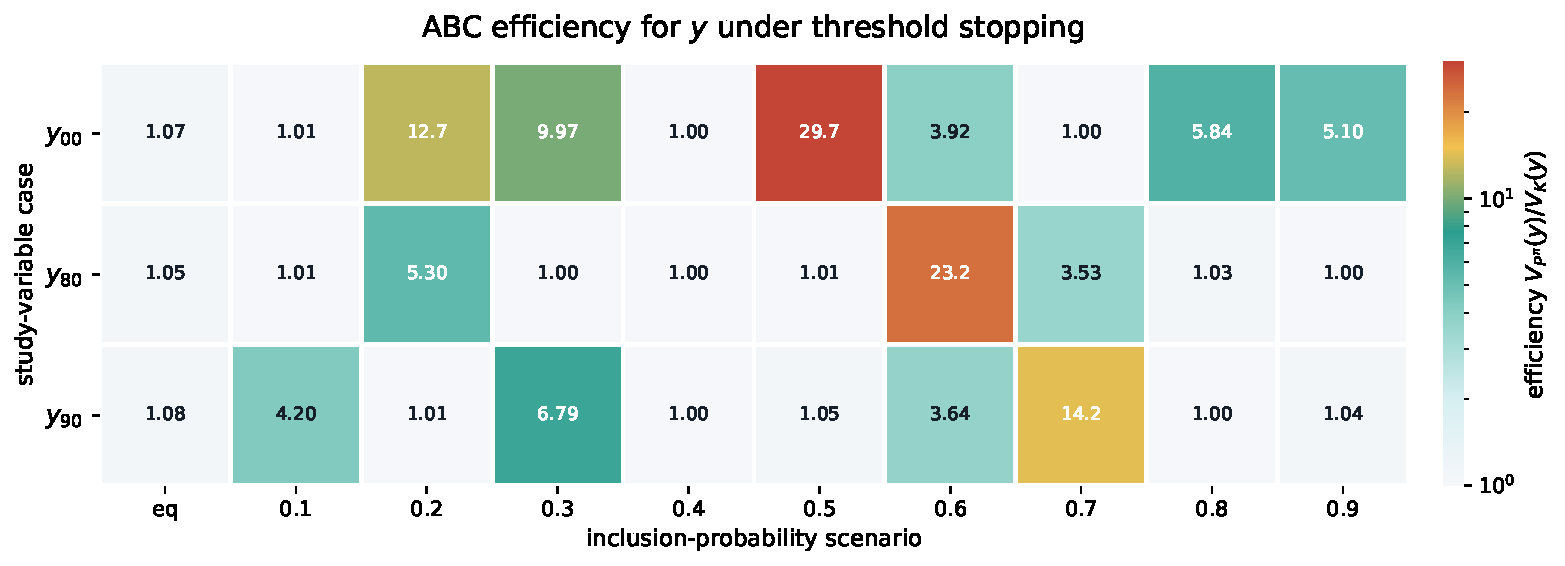
\includegraphics[width=0.95\textwidth]{abc_threshold_efficiency_heatmap_pretty.pdf}
\caption{Efficiency for the optimized variable \(z\) under threshold stopping. Each cell reports \(V_{\Ppi_z}(z)/V_K(z)\). Light cells close to one indicate that no meaningful improvement over the real-valued \(\Ppi\) reference was found. Colored cells indicate scenarios where ABC found a candidate complex kernel with smaller computed HT variance.}
\label{fig:abc-threshold-efficiency}
\end{figure}

\begin{figure}[!htbp]
\centering
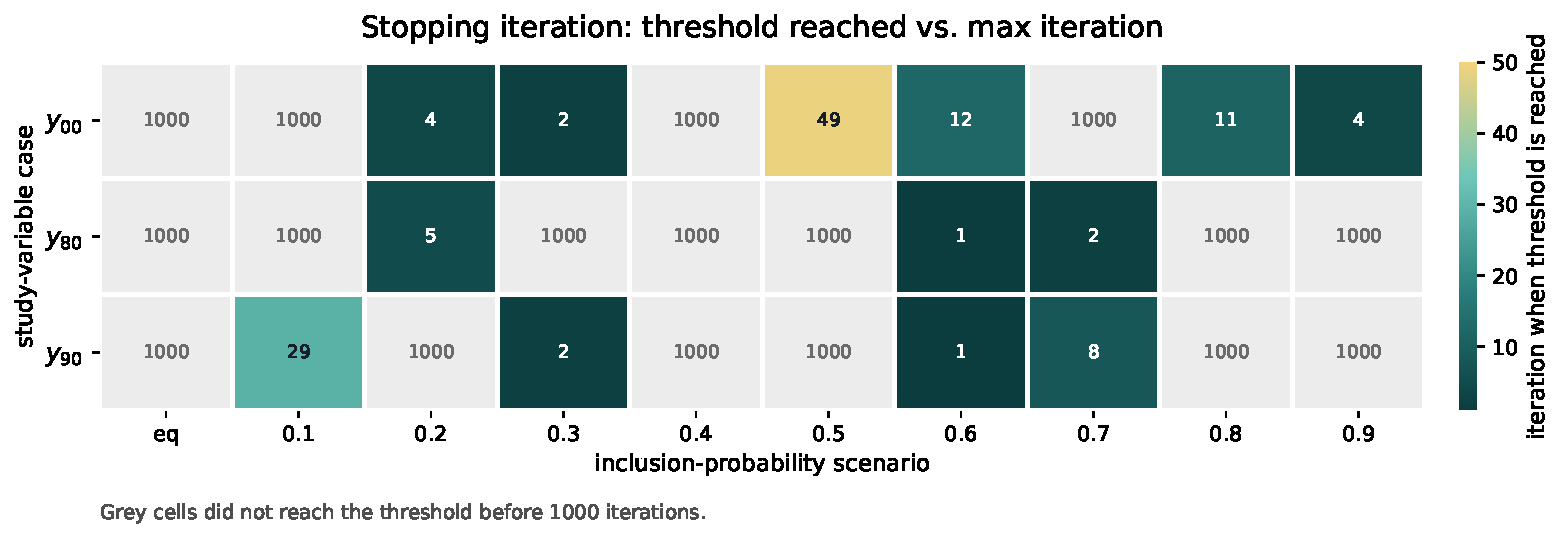
\includegraphics[width=0.95\textwidth]{abc_threshold_stop_iteration_heatmap_pretty.pdf}
\caption{Iteration at which the search stopped. Colored cells reached the \(z\)-efficiency threshold before \(1000\) iterations; the number is the first reported stopping iteration. Grey cells did not reach the threshold and therefore stopped at the maximum iteration limit.}
\label{fig:abc-threshold-stopping}
\end{figure}

Figures~\ref{fig:abc-threshold-efficiency} and~\ref{fig:abc-threshold-stopping} summarize the optimization results for \(z\). In 13 of the 30 scenarios, ABC reaches the threshold before the maximum iteration limit. Several of these improvements occur very quickly, sometimes within only a few iterations. In the remaining scenarios, the efficiency remains close to one even after \(1000\) iterations. This suggests two qualitatively different regimes: some combinations of \(z\) and \(\pi\) allow the complex CaDSD parametrization to improve rapidly on the real-valued reference, while others appear much more resistant to improvement.

\begin{figure}[!htbp]
\centering
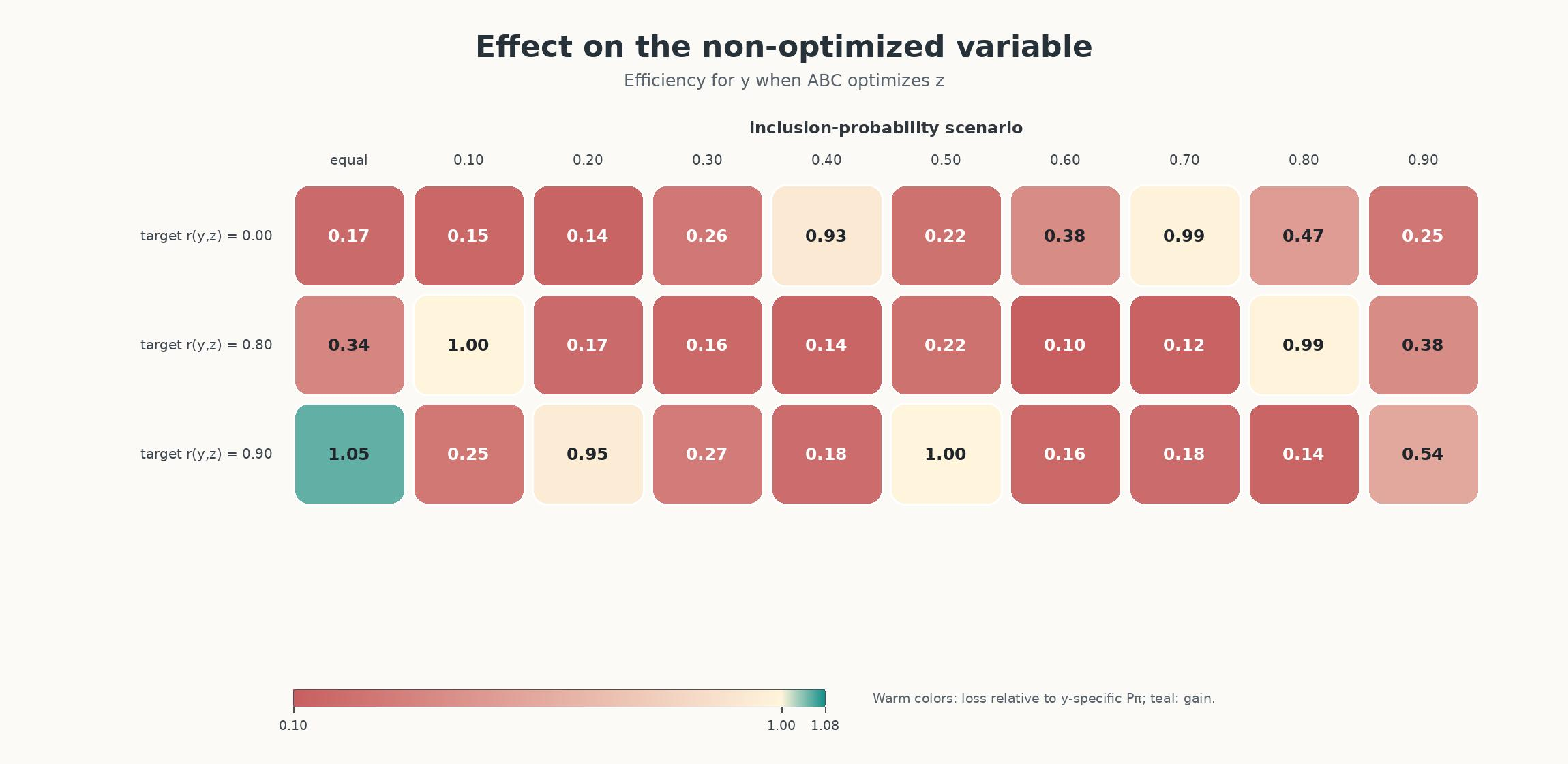
\includegraphics[width=0.95\textwidth]{abc_threshold_auxiliary_efficiency_heatmap_pretty.pdf}
\caption{Effect of the \(z\)-optimized kernel on the companion variable \(y\). Each cell reports \(V_{\Ppi_y}(y)/V_K(y)\), where \(\Ppi_y\) is the Vincent reference built from the \(y/\pi\) ordering. Values below one show that the \(z\)-optimized kernel is worse than the \(y\)-specific real-valued reference for estimating \(y\).}
\label{fig:abc-auxiliary-efficiency}
\end{figure}

\begin{figure}[!htbp]
\centering
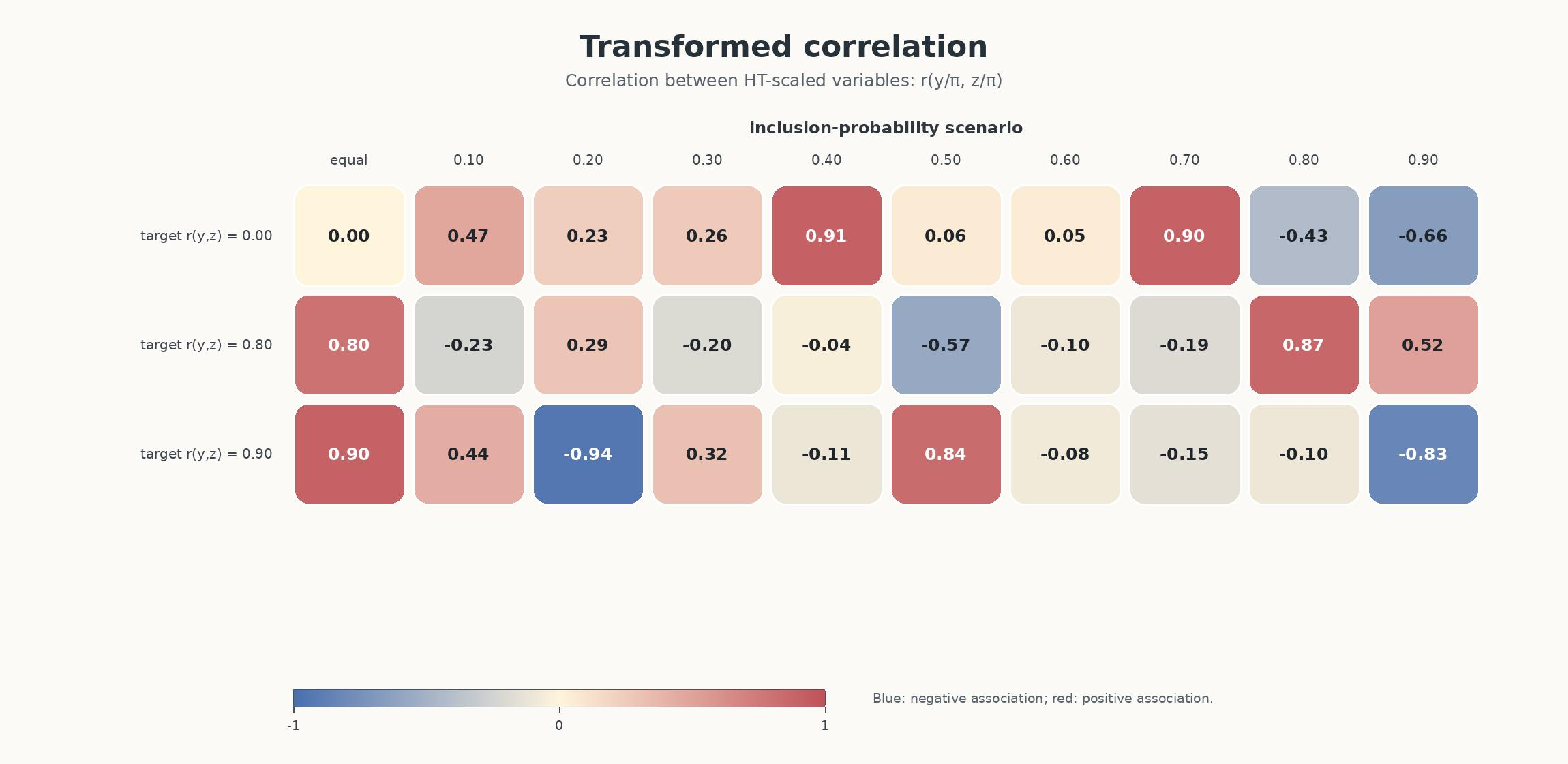
\includegraphics[width=0.95\textwidth]{abc_threshold_transformed_correlation_heatmap_pretty.pdf}
\caption{Correlation between the HT-scaled variables \(y/\pi\) and \(z/\pi\). The raw correlation \(r(y,z)\) is fixed by row, but the transformed correlation can change substantially once the inclusion probabilities are introduced.}
\label{fig:abc-transformed-correlation}
\end{figure}

Figures~\ref{fig:abc-auxiliary-efficiency} and~\ref{fig:abc-transformed-correlation} explain why improvement for \(z\) does not automatically transfer to \(y\). Even when the raw correlation \(r(y,z)\) is high, the transformed correlation \(r(y/\pi,z/\pi)\) can be weak or negative. Since the HT variance is driven by the scaled quantities, optimizing the design for \(z\) can leave the variance for \(y\) almost unchanged or make it worse relative to the \(y\)-specific Vincent reference. This is visible in Figure~\ref{fig:abc-auxiliary-efficiency}: most cells are below one, with only a few cases near or slightly above one.

The results should still be interpreted as numerical evidence rather than as a theoretical optimum. They show that, under the CaDSD parametrization and the numerical checks used in the notebook, ABC can find complex Hermitian kernels with the prescribed diagonal and smaller computed HT variance for the optimized variable \(z\) than the real-valued \(\Ppi\) reference. The auxiliary-variable heatmap shows that this gain is target-specific. The candidate kernels should be checked independently for admissibility, projection accuracy, and variance calculation before making a final claim.

\section{Conclusion}

This experiment focuses on an optimized variable \(z\), a companion variable \(y\), and several inclusion-probability vectors satisfying Vincent's monotonicity condition for \(z\). The CaDSD Vincent start reproduces the real-valued \(\Ppi\) reference variance as expected. When ABC is allowed to move in the complex CaDSD parametrization, it finds candidate kernels that substantially reduce the computed HT variance for \(z\) in several scenarios. The auxiliary analysis shows that these improvements are target-specific and do not automatically transfer to \(y\).

The results are promising but should be treated as numerical evidence rather than a final theoretical claim. The next step is to verify the exported complex kernels independently, especially the cases with very large efficiency values, and then repeat the experiment with stronger projection tolerances and additional populations.

\begin{thebibliography}{99}

\bibitem[Basturk and Karaboga(2006)]{BasturkKaraboga2006}
Basturk, B. and Karaboga, D. (2006).
An artificial bee colony algorithm for numeric function optimization.
In \emph{Proceedings of the IEEE Swarm Intelligence Symposium}, Indianapolis, USA.

\bibitem[Deville and Till\'{e}(2004)]{DevilleTille2004}
Deville, J.-C. and Till\'{e}, Y. (2004).
Efficient balanced sampling: The cube method.
\emph{Biometrika}, 91(4), 893--912.

\bibitem[Horvitz and Thompson(1952)]{HorvitzThompson1952}
Horvitz, D. G. and Thompson, D. J. (1952).
A generalization of sampling without replacement from a finite universe.
\emph{Journal of the American Statistical Association}, 47(260), 663--685.

\bibitem[Karaboga(2005)]{Karaboga2005}
Karaboga, D. (2005).
An idea based on honey bee swarm for numerical optimization.
Technical Report TR06, Erciyes University, Engineering Faculty, Computer Engineering Department.

\bibitem[Karaboga and Akay(2009)]{KarabogaAkay2009}
Karaboga, D. and Akay, B. (2009).
A comparative study of artificial bee colony algorithm.
\emph{Applied Mathematics and Computation}, 214(1), 108--132.

\bibitem[Karaboga and Basturk(2007)]{KarabogaBasturk2007}
Karaboga, D. and Basturk, B. (2007).
A powerful and efficient algorithm for numerical function optimization: Artificial bee colony algorithm.
\emph{Journal of Global Optimization}, 39, 459--471.

\bibitem[Loonis(2023)]{Loonis2023}
Loonis, V. (2023).
Constructing all determinantal sampling designs.
\emph{Survey Methodology}, 49(2), 411--441.

\bibitem[Loonis and Mary(2019)]{LoonisMary2019}
Loonis, V. and Mary, X. (2019).
Determinantal sampling designs.
\emph{Journal of Statistical Planning and Inference}, 199, 60--88.

\end{thebibliography}

\end{document}
